\chapter{Códigos de Correção de Erro}

Um dos principais resultados visto anteriormente, conhecido como o segundo teorema de
Shannon, afirma que, para taxas de transmissão $R$ inferiores à capacidade
do canal $C$, existe uma sequência de códigos capaz de reduzir a
probabilidade de erro a zero, desde que o tamanho dos blocos codificados seja
suficientemente grande. Em termos matemáticos, se $R < C$, é possível
projetar códigos que, com o aumento do comprimento do bloco, garantem uma
transmissão praticamente livre de erros. No entanto, esse teorema é um
resultado de existência: ele não especifica como construir tais códigos, nem
considera as limitações práticas de implementação, como a complexidade
computacional ou os recursos físicos disponíveis.

Na prática, a codificação baseada em sequências típicas, que aproxima o limite
teórico de Shannon, exige blocos de tamanho exponencialmente grande, o que é
inviável para a maioria das aplicações reais. Para superar esse desafio,
recorremos aos códigos de correção de erro, que introduzem redundância
controlada às mensagens, permitindo não apenas a detecção, mas também a
correção de erros causados pelo ruído no canal. Esses códigos são projetados
para equilibrar eficiência (taxa de transmissão) e robustez (capacidade de
correção), tornando a comunicação confiável mesmo em condições adversas.

Os códigos de correção de erro podem ser classificados em dois grandes grupos.
Os códigos de bloco transformam mensagens de $k$-bits em
palavras-código de $n$-bits, com $n > k$, sem depender de transmissões
anteriores. Exemplos incluem o código de Hamming, amplamente utilizado em
memórias RAM para proteger dados contra erros, e o código Reed-Solomon,
essencial em tecnologias como CDs, DVDs, códigos QR e comunicações espaciais,
como as missões Voyager e Galileo. Já os códigos convolucionais operam
como máquinas de estado finito, gerando saídas que dependem tanto da entrada
atual quanto de estados anteriores. Um exemplo proeminente é o código Turbo,
que desempenha um papel crucial em comunicações móveis modernas, como 3G, 4G e
LTE.

Além da abordagem baseada em codificação, a confiabilidade da comunicação pode
ser melhorada por meios físicos, como o aumento da potência de transmissão, o
uso de componentes eletrônicos com menor tolerância ao ruído ou a redução de
interferências ambientais, como ruído térmico ou poeira. Contudo, essas
soluções frequentemente elevam os custos ou a complexidade do sistema, tornando
os códigos de correção de erro uma alternativa mais elegante e eficiente. Em
muitos casos, é a combinação de codificação inteligente e otimizações físicas
que garante o sucesso de sistemas de comunicação modernos.






\section{Distância de Hamming}

Para projetar códigos de correção de erro eficazes, precisamos de uma métrica
que quantifique quão diferentes são as palavras-código de um código. Essa
métrica é conhecida como distância de Hamming, um conceito central na
teoria dos códigos.

\begin{definition}[Distância de Hamming]
A \emph{distância!de Hamming}\index{distância de Hamming} entre duas sequências de mesmo comprimento, definidas 
sobre um alfabeto finito qualquer, é o número de
posições em que elas diferem. Formalmente, para duas palavras 
$x = (x_1, x_2, \dots, x_n)$ e $y = (y_1, y_2, \dots, y_n)$, a distância de Hamming é
dada por:
\begin{equation}
d_H(x, y) = |\{ i : x_i \neq y_i \}|.
\end{equation}
\end{definition}


\begin{example}[Distância de Hamming para sequências binárias]
Por exemplo, considere as palavras-código binárias $x = 10110$ e 
$y = 11011$. Para sequências binárias, podemos calcular a distância de Hamming
usando a operação XOR bit a bit, que resulta em 1 nas posições onde os bits
diferem, e então contar o número de 1s. Comparando posição por posição:
\[
\begin{array}{r|ccccc}
x & 1 & 0 & 1 & 1 & 0 \\
y & 1 & 1 & 0 & 1 & 1 \\
\hline
x \oplus y & 0 & 1 & 1 & 0 & 1 \\
\end{array}
\]
O resultado do XOR é $01101$, com 1s nas posições 2, 3 e 5, 
indicando que essas posições diferem. Assim, $d_H(x, y) = 3$.
\end{example}


\begin{example}[Distância de Hamming para alfabeto não binário]
Para um alfabeto não binário, considere as sequências $u = (0, 1, 2, 0)$ e
$v = (0, 2, 2, 1)$ sobre o alfabeto $\{0, 1, 2\}$. Comparamos cada posição: 
$u_1 = v_1 = 0$ (iguais), $u_2 = 1 \neq v_2 = 2$, $u_3 = 2 = v_3 = 2$, 
$u_4 = 0 \neq v_4 = 1$. As posições 2 e 4 diferem, logo $d_H(u, v) = 2$.
\end{example}



\begin{definition}[Distância mínima de um código]
Para um código $C$, composto por um conjunto de palavras-código, a \emph{distância
mínima}\index{distância!mínima} $d_{\text{min}}$ é definida como a menor distância de Hamming entre
quaisquer duas palavras-código distintas:
\begin{equation}
d_{\text{min}} = \min \{ d_H(x, y) : x, y \in C, x \neq y \}.
\end{equation}
\end{definition}

A distância mínima é um parâmetro fundamental, pois determina a capacidade do
código de detectar e corrigir erros, como estabelecido pelos seguintes
teoremas.

\begin{theorem}[Detecção de Erros]\label{thm:deteccaoerros}\index{teorema!detecção de erros}
Um código $C$ com distância mínima $d_{\text{min}}$ pode detectar até $d_{\text{min}} - 1$ erros em qualquer palavra-código.
\end{theorem}
\begin{proof}
Suponha que uma palavra-código $c \in C$ seja transmitida e receba até $k$ erros,
resultando em uma sequência $r$, tal que $d_H(c, r) \leq k$.
Para que o erro seja detectado, $r$ não deve ser uma palavra-código válida,
ou seja, $r \notin C$. Como $d_{\text{min}}$ é a menor distância entre quaisquer
duas palavras-código distintas, para qualquer $c' \in C$, com $c' \neq c$, 
temos $d_H(c, c') \geq d_{\text{min}}$. Se $k \leq d_{\text{min}} - 1$, então:
\begin{equation}
d_H(c, r) \leq d_{\text{min}} - 1 < d_{\text{min}}.
\end{equation}
Assim, $r$ não pode ser igual a nenhuma outra palavra-código $c'$, pois 
$d_H(c, r) < d_H(c, c')$. Portanto, $r \notin C$, e o erro é detectado.
Se $k = d_{\text{min}}$, $r$ poderia ser igual a outra palavra-código,
e o erro não seria detectado. Logo, o código é capaz de detectar até $d_{\text{min}} - 1$ erros.
\end{proof}

\begin{theorem}[Correção de Erros]\label{thm:correcaoerros}\index{teorema!correção de erros} 
Um código $C$ com distância mínima $d_{\text{min}}$ pode corrigir até
$t = \lfloor (d_{\text{min}} - 1)/2 \rfloor$ erros em qualquer palavra-código.
\end{theorem}

\begin{proof}
Para corrigir erros, o decodificador deve identificar a palavra-código $c \in C$
mais próxima da sequência recebida $r$, segundo a distância de Hamming 
(decodificação por máxima verossimilhança). Considere esferas de Hamming de raio $t$
centradas em cada palavra-código (veja a \Cref{fig:hammingspheres}), 
onde a esfera em torno de $c$ contém todas as sequências $r$ 
tais que $d_H(c, r) \leq t$. Para que o código corrija até $t$ erros, essas esferas não 
devem se sobrepor, garantindo que $r$ esteja na esfera de uma única palavra-código.

Seja $t = \lfloor (d_{\text{min}} - 1)/2 \rfloor$. Suponha que $r$ está à distância
$\leq t$ de $c$, ou seja, $d_H(c, r) \leq t$, devido a ocorrência de até $t$ erros em $r$. Para qualquer
outra palavra-código $c' \neq c$, temos $d_H(c, c') \geq d_{\text{min}}$. 
Queremos garantir que $r$ não esteja na esfera de $c'$, ou seja, $d_H(c', r) > t$.
Pela desigualdade triangular:
\begin{equation}
d_H(c', r) \geq d_H(c, c') - d_H(c, r) \geq d_{\text{min}} - t.
\end{equation}
Substituindo $t = \lfloor (d_{\text{min}} - 1)/2 \rfloor$, temos:
\begin{subequations}
\begin{align}
  d_{\text{min}} - t &= d_{\text{min}} - \lfloor (d_{\text{min}} - 1)/2 \rfloor \\
                     &\geq d_{\text{min}} - (d_{\text{min}} - 1)/2 \label{dem:corerresfertA}\\
                     &= (d_{\text{min}} + 1)/2 \\
                     &> t,
\end{align}
\end{subequations}
onde em \ref{dem:corerresfertA} utilizamos que $\lfloor x \rfloor \leq x$.
Assim, $d_H(c', r) > t$, e $r$ está na esfera de apenas uma palavra-código, 
permitindo corrigir até $t$ erros. Se o número de erros fosse $t + 1$, as esferas
poderiam se sobrepor, levando a erros de decodificação. 
Portanto, o código corrige até $t$ erros.
\end{proof}

\begin{marginfigure}
    \centering
    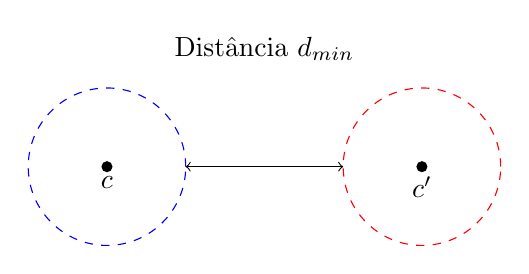
\begin{tikzpicture}
        % Esferas de Hamming
        \fill[black] (0,0) circle (2pt) node[below] {$c$};
        \draw[blue, dashed] (0,0) circle (1cm);
        \fill[black] (4,0) circle (2pt) node[below] {$c'$};
        \draw[red, dashed] (4,0) circle (1cm);
        \node at (2,1.5) {Distância $d_{\text{min}}$};
        \draw[<->] (1,0) -- (3,0);
    \end{tikzpicture}
    \caption{Esferas de Hamming de raio $t = \lfloor (d_{\text{min}} - 1)/2 \rfloor$. As palavras-código $c$ e $c'$ estão separadas por $d_{\text{min}}$, garantindo que erros de até $t$ símbolos sejam corrigidos.}\label{fig:hammingspheres}
\end{marginfigure}



\begin{example}[Correção de erros em um código de repetição com $n=3$]\index{código!de repetição}
Considere um código simples com palavras-código $\{000, 111\}$ sobre o
alfabeto binário. A distância de Hamming entre $000$ e $111$ é 3, logo
$d_{\text{min}} = 3$. Pelo \hyperref[thm:deteccaoerros]{Teorema de Detecção de Erros}, esse código
detecta até $3 - 1 = 2$ erros. Pelo \hyperref[thm:correcaoerros]{Teorema de Correção de Erros}, ele
corrige até $\lfloor (3 - 1)/2 \rfloor = 1$ erro. Se recebermos $001$,
sabemos que houve erro (pois $001 \notin C$) e corrigimos para $000$,
que está a distância 1. Note que, para obter a sequência $111$ deveríamos
considerar a ocorrência de dois erros, neste caso, é menos provável
que dois erros tenham ocorrido do que apenas um. A decodificação
de máxima verossimilhança escolhe a alternativa mais verossímel, no caso,
a sequência $000$.
\end{example}


A distância de Hamming está diretamente ligada à
redundância\index{redundância} do código: adicionar mais símbolos (aumentando $n$) permite
maior separação entre palavras-código, mas reduz a taxa $R = k/n$. 
Existe então uma relação de compromisso entre aumentar $d_{\text{min}}$ e
redzir $R$.







\section{Código de Repetição}\label{sec:codrepeticao}

O código de repetição é o exemplo mais simples de um código de correção de
erro. Apesar de sua simplicidade, ele ilustra o papel da redundância e serve
como ponto de partida para entender outros códigos.

\begin{definition}[Código de repetição]
Um \emph{código de repetição}\index{código!de repetição} com parâmetro $n$ codifica cada bit da mensagem repetindo-o $n$ vezes. 
Para uma mensagem de 1 bit:
\begin{equation}
0 \mapsto \underbrace{00\dots0}_{n \text{ vezes}}, \quad 1 \mapsto \underbrace{11\dots1}_{n \text{ vezes}}.
\end{equation}
Um código de repetição terá taxa $R = 1/n$, distância mínima $d_{\text{min}} = n$
e será capaz de corrigir até $t = \lfloor (d_{\text{min}} - 1)/2 \rfloor = \lfloor (n - 1)/2 \rfloor$ bits.
\end{definition}


\begin{example}[Correção de erros em um código de repetição com $n=3$]
  Revisitando o exemplo anterior, um código de repetição com $n=3$,
  terá a seguinte tabela de codificação:
  \begin{table}[h]
    \centering
    \begin{tabular}{lll}
      mensagem & 0 & 1 \\
      palavra-código & 000 & 111 
    \end{tabular}
    \caption{Código de repetição com $n = 3$.}
    \label{tab:repetition_code}
  \end{table}

  \noindent A mensagem $10$, por exemplo, será codificada como $10 \mapsto 111000$.
  A decodificação é feita por regra/voto de maioria. 
  Para cada bloco de $n$ bits, escolhemos o bit mais frequente. 
  Por exemplo, se $n = 3$ e recebemos $011$, contamos dois 1s e um 0, 
  decodificando como 1 (palavra-código $111$).
  Este código terá uma taxa de $R = 1/3$, distância mínima $d_{\text{min}} = 3$ e
  poderá corrigir apenas 1 bit.
\end{example}


Embora o código de repetição seja fácil de implementar, sua baixa taxa o torna
ineficiente para aplicações práticas. 
Através da análise deste código simples, foi possível verificar a
relação entre redundância e distância de Hamming. Aumentar $n$ eleva 
$d_{\text{min}}$, melhorando a correção de erros, mas reduz drasticamente a taxa. 








\section{Código de Verificação de Paridade Simples}

O \emph{código de verificação de paridade simples}\index{código!de verificação de paridade} consiste em adicionar um único bit
de redundância a uma mensagem binária, permitindo detectar certos tipos de
erros, embora não seja capaz de corrigi-los. Este código serve como base para
muitos esquemas de codificação, como o código de Hamming e os códigos de
verificação de paridade de baixa densidade (LDPC).

\begin{definition}[Código de verificação de paridade simples]
O código de verificação de paridade simples opera com entrada e saída binárias, ou seja, 
$\mathcal{X} = \mathcal{Y} = \{0, 1\}$. Uma mensagem de $n-1$ bits, denotada $x_{1:n-1} = (x_1, x_2, \dots, x_{n-1})$, 
é codificada em uma palavra-código de $n$ bits, onde os primeiros $n-1$ são iguais àqueles da mensagem original
e o $n$-ésimo bit, chamado bit de paridade, é definido como:
\begin{equation}
x_n = \mod \left( \sum_{i=1}^{n-1} x_i, 2 \right).
\end{equation}
Assim, $x_n = 0$ se o número de 1s em $x_{1:n-1}$ for par, e $x_n = 1$ se for ímpar, 
garantindo que a soma total de 1s na palavra-código $(x_1, x_2, \dots, x_n)$ seja par.
\end{definition}

Uma palavra-código $(x_1, x_2, \dots, x_n)$ é considerada válida se satisfizer a condição de paridade:
\begin{equation}
\mod \left( \sum_{i=1}^{n} x_i, 2 \right) = 0.
\end{equation}
Essa condição implica que o número total de 1s na palavra-código é par. Durante
a transmissão, se um número ímpar de bits for alterado (ou seja, se ocorrer um
número ímpar de erros), essa soma deixará de ser par, permitindo a detecção do
erro. No entanto, um número par de erros manterá a soma par, passando
despercebido.

\begin{theorem}[Detecção de Erros por Paridade]\index{teorema!detecção de erros por paridade}
O código de verificação de paridade simples detecta qualquer número ímpar de
erros em uma palavra-código, mas não detecta um número par de erros.
\end{theorem}
\begin{proof}
Considere uma palavra-código válida $c = (c_1, c_2, \dots, c_n)$, onde
$\mod \left( \sum_{i=1}^{n} c_i, 2 \right) = 0$. Suponha que $k$ bits
sejam alterados devido a erros, resultando em uma sequência recebida 
$r = (r_1, r_2, \dots, r_n)$. Cada erro inverte um bit ($0 \to 1$ ou $1 \to 0$), 
alterando a soma dos bits em $\mod(k, 2)$. Dessa forma:
\begin{equation}
\mod \left( \sum_{i=1}^{n} r_i \right) = \mod \left( \sum_{i=1}^{n} c_i \right) + k \mod 2.
\end{equation}
Como $\sum_{i=1}^{n} c_i \mod 2 = 0$, temos:
\begin{equation}
\mod \left( \sum_{i=1}^{n} r_i, 2 \right) = \mod(k, 2).
\end{equation}
Se $k$ é ímpar, $\mod(k, 2) = 1$, e a soma dos bits de $r$ será ímpar, 
violando a condição de paridade e indicando um erro. Se $k$ é par, 
$\mod(k, 2) = 0$, e a soma permanece par, fazendo $r$ parecer uma 
palavra-código válida, mesmo que contenha erros. 
Portanto, o código detecta apenas um número ímpar de erros.
\end{proof}

\begin{example}[Verificação de paridade simples]\label{ex:simplyparitycheck}
Considere um codificador $E: \{0, 1\}^3 \to \{0, 1\}^4$, definido por:
\begin{equation}
E(x_1, x_2, x_3) = \left( x_1, x_2, x_3, \mod(x_1 + x_2 + x_3, 2) \right).
\end{equation}
As palavras-código são todas as sequências de 4 bits com um número par de 1s:
\[
C = \{ (0,0,0,0), (0,0,1,1), (0,1,0,1), (0,1,1,0), (1,0,0,1), (1,0,1,0), (1,1,0,0), (1,1,1,1) \}.
\]
A tabela \ref{tab:paritycode} lista as mensagens e suas respectivas palavras-código.

  \begin{table}[h]
    \centering
    \begin{tabular}{cc}
        \toprule
        Mensagem $(x_1, x_2, x_3)$ & Palavra-código $(x_1, x_2, x_3, x_4)$ \\
        \midrule
        (0,0,0) & (0,0,0,0) \\
        (0,0,1) & (0,0,1,1) \\
        (0,1,0) & (0,1,0,1) \\
        (0,1,1) & (0,1,1,0) \\
        (1,0,0) & (1,0,0,1) \\
        (1,0,1) & (1,0,1,0) \\
        (1,1,0) & (1,1,0,0) \\
        (1,1,1) & (1,1,1,1) \\
        \bottomrule
    \end{tabular}
    \caption{Código de verificação de paridade simples com $n = 4$.}
    \label{tab:paritycode}
\end{table}

Suponha que a palavra-código $(0,1,0,1)$ seja transmitida. Vamos analisar dois cenários: apagamento e erro.
Para o caso de apagamento, suponha que a sequência recebida seja $r = (0, \text{x}, 0, 1)$, 
onde o segundo bit foi apagado. Calculamos a soma dos bits conhecidos: $0 + 0 + 1 = 1 \mod 2$.
Para que $r$ seja válida, a soma total deve ser par, logo o bit apagado deve ser 1 (pois $1 + 1 = 0 \mod 2$). 
Assim, reconstruímos $r = (0,1,0,1)$, recuperando a palavra-código correta.
Agora, paa o caso de erro, suponha que a sequência recebida seja $r = (0,0,0,1)$. 
Calculamos a soma: $0 + 0 + 0 + 1 = 1 \mod 2$, que é ímpar. 
Como a soma viola a condição de paridade, detectamos que houve um erro 
(neste caso, um erro no segundo bit, pois $(0,1,0,1) \to (0,0,0,1)$).
Se a sequência recebida fosse $r = (0,0,0,0)$ (decorrente de dois erros, nos bits 2 e 4), 
a soma seria $0 + 0 + 0 + 0 = 0 \mod 2$, indicando paridade válida. 
No entanto, como $(0,0,0,0) \neq (0,1,0,1)$, houve dois erros que não foram detectados,
confirmando que o código falha para um número par de erros.
\end{example}

A distância mínima do código de paridade é $d_{\text{min}} = 2$. 
Duas palavras-código diferem ao menos em 1 bit dentre os primeiros $n-1$ bits,
por serem palavras diferentes. Além disso, neste caso, elas devem também diferir
no bit paridade, fazendo com que $d_{\text{min}} = 2$. Note que, o bit de 
paridade de duas palavras distintas pode ser o mesmo, desde que as duas palavras
tenham ao menos dois bits distintos entre os primeiros $n-1$ bits. 
De qualquer forma, teremos $d_{\text{min}} = 2$.

Pelo \hyperref[thm:deteccaoerros]{teorema de detecção de erros},  
um código com $d_{\text{min}} = 2$ detecta até $1$ erro, o que é consistente com
nossa análise: um erro (ímpar) viola a paridade, mas dois erros (par) não são
detectados. Para correção, usando o \hyperref[thm:correcaoerros]{teorema de correção de erros}, 
temos $t = \lfloor (d_{\text{min}} - 1)/2 \rfloor = 0$,
indicando que o código não corrige erros, apenas os detecta.

O código de verificação de paridade simples é limitado, pois não corrige erros
e falha em detectar erros pares. No entanto, sua simplicidade o torna útil em
aplicações como memórias de computadores e comunicações básicas, onde a
detecção de erros é suficiente. Ele ainda é a base para outros códigos,
como por exenplo, o código de Hamming. 





\section{Definição de Códigos [n, k, d]}

Na teoria dos códigos de correção de erros, é comum descrever um código por
meio de três parâmetros que resumem suas propriedades essenciais.
Essa notação, conhecida como \emph{códigos [n, k, d]}\index{código![n,k,d]}, fornece uma maneira
concisa de caracterizar a estrutura e a capacidade de um código, permitindo
comparar diferentes esquemas de codificação.

\begin{definition}[Códigos $\lbrack n,k,d \rbrack$]\label{def:codnkd}
Um \emph{código [n, k, d]} é um código de correção de erros linear com as seguintes características:
possui comprimento de palavra de código $n$ (incluindo os bits de dados e os bits de redundância);
possui $k$ bits de dados (tamanho da mensagem antes da codificação);
e com distância mínima de Hamming $d$ entre quaisquer duas palavras-código distintas do código.
\end{definition}

Como discutido anteriormente, a distância mínima $d_{\text{min}}$ determina
diretamente a capacidade de um código de lidar com erros. 
Utilizando resultados já estabelecidos anteriormente, podemos concluir que um 
código [n, k, d] pode detectar até \( d - 1 \) erros, pois qualquer alteração de até $d - 1$ 
símbolos em uma palavra-código não a transforma em outra palavra-código válida;
corrigir até $\lfloor (d - 1)/2 \rfloor$ erros, 
pois esferas de Hamming de raio $\lfloor (d - 1)/2 \rfloor$ centradas nas palavras-código 
não se sobrepõem, garantindo que a palavra-código correta seja identificada.

A taxa do código, definida como $R = k/n$, mede a eficiência do código: 
quanto maior $k$ em relação a $n$, menos redundância e maior a taxa, 
mas isso pode reduzir $d$, comprometendo a capacidade de correção. 
O desafio no projeto de códigos é maximizar $d$ e $k$ para um dado $n$.

Data a \Cref{def:codnkd}, podemos agora caracterizar os códigos vistos anteriormente como:
código de repetição com $n=3$ (mensagem de 1 bit repetida três vezes)  é um código [3, 1, 3];
código de paridade simples com $n=4$ é um código [4, 3, 2].


\begin{definition}[Código Linear]
Um \emph{código linear}\index{código!linear} $\mathcal{C}$ de comprimento $n$ sobre um corpo $\mathbb{F} = \text{GF}(q)$ 
(onde $q$ é geralmente uma potência de um primo) é um subespaço vetorial de $\mathbb{F}^n$ sobre $\mathbb{F}$.
Em outras palavras, $\mathcal{C} \subseteq \mathcal{F}^n$ é um código linear se, para quaisquer palavras-código 
$\mathbf{c}_1, \mathbf{c}_2 \in \mathcal{C}$, e quaisquer escalares $\alpha, \beta \in \mathbb{F}$, temos:
$\alpha \mathbf{c}_1 + \beta \mathbf{c}_2 \in \mathcal{C}$, onde as operações de soma e multiplicação por escalar 
são definidas componente a componente no corpo finito $\mathbb{F}_q$. 
Para um código binário ($q = 2$), $\mathbb{F} = \{0, 1\}$, e a soma é feita módulo 2.

Um código linear $\mathcal{C}$ com $k$ dimensões (ou seja, $|\mathcal{C}| = q^k$) pode ser descrito 
por uma matriz geradora $\mathbf{G}$ de tamanho $k \times n$, onde cada palavra-código é da forma 
$\mathbf{v} \mathbf{G}$, com $\mathbf{v} \in \mathbb{F}^k$. 
Alternativamente, $C$ é o espaço nulo de uma matriz de verificação de paridade $\mathbf{H}$ de tamanho 
$(n-k) \times n$, tal que $\mathbf{H} \mathbf{c} = \mathbf{0}$ para toda palavra $\mathbf{c} \in \mathcal{C}$.
\end{definition}


Se $\mathcal{C}$ é um código linear $(n,M,d)$ sobre $\mathbb{F}$ e a dimensionalidade de $\mathcal{C}$ é $k$,
então dizemos que $\mathcal{C}$ é um código linear $[n,k,d]$ sobre $\mathbb{F}$. A diferença $n-k$ é a 
redundância do código. Toda base de um código linear $[n,k,d]$ $\mathcal{C}$ sobre $\mathbb{F} = \text{GF}(q)$
contém $k$ palavras distintas que geram todo o código $\mathcal{C}$ por combinações lineares delas.
Assim, $\vert\mathcal{C}\vert = M = q^k$ e a taxa do código é $R = \sfrac{\log_q M}{n} = k/n$.
As linhas da matriz geradora $\mathbf{G}$ serão a base do código (podendo não ser úncia).


\begin{definition}[Peso de Hamming]
O \emph{peso de Hamming}\index{código!peso da palavra} de uma palavra $\mathbf{c} \in \mathcal{C}$
é o número de posições em que $\mathbf{c}$ tem elementos não nulos, ou seja:
\begin{equation}
  w(\mathbf{c}) = |\{ i \in \{1, 2, \dots, n\} : c_i \neq 0 \}|,
\end{equation}
onde $\mathbf{c} = (c_1, c_2, \dots, c_n)$. 
Para um código binário ($\mathcal{X} = \{0, 1\}$), o peso de Hamming é simplesmente o número de 1s na palavra. 

\begin{example}
Considere $\mathbf{c} = (1, 0, 1, 1, 0)$ em um código binário ($q = 2$, $n = 5$). 
O peso de Hamming é: $w(\mathbf{c}) = |\{1, 3, 4\}| = 3$,
pois $\mathbf{c}$ tem 1s nas posições 1, 3 e 4.
\end{example}
\end{definition}

\begin{definition}[Peso mínimo de um código]
O \emph{peso mínimo de um código}\index{código!peso mínimo} $\mathcal{C} \subseteq \mathbb{F}^n$, 
onde $\mathcal{X} = \{0, 1, \dots, q-1\}$ é um alfabeto $q$-ário, 
é o menor peso de Hamming entre todas as palavras-código não nulas de $\mathcal{C}$, ou seja:
\begin{equation}
w_{\text{min}}(\mathcal{C}) = \min \{ w(\mathbf{c}) : \mathbf{c} \in \mathcal{C}, \mathbf{c} \neq \mathbf{0} \},
\end{equation}
onde $w(\mathbf{c})$ é o peso de Hamming de $\mathbf{c}$, 
conforme definido anteriormente. 
%Para um código linear, o peso mínimo é igual à distância mínima 
%$d_{\text{min}}$ do código, pois $d_H(\mathbf{c}_1, \mathbf{c}_2) = w(\mathbf{c}_1 - \mathbf{c}_2) \), e \( \mathbf{c}_1 - \mathbf{c}_2 \in C \) devido à linearidade. Assim, para um código linear, o menor peso de uma palavra não nula determina a capacidade de detecção (\( d_{\text{min}} - 1 \)) e correção (\( \lfloor (d_{\text{min}} - 1)/2 \rfloor \)) de erros.
\end{definition}


\begin{proposition}[Distância e peso mínimo]
Seja $\mathcal{C}$ um código linear $[n,k,d]$ sobre $\mathbb{F}$, então
\begin{equation}
	  d = \min_{\mathbf{c} \in \mathcal{C} \backslash \{\mathbf{0}\}}  w(\mathbf{c}) .
\end{equation}
\end{proposition}
\begin{proof}
Como $\mathcal{C}$ é linear, dadas duas palavras $\mathbf{c}_1, \mathbf{c}_2 \in \mathcal{C}$, teremos
que $\mathbf{c}_1 - \mathbf{c}_2 \in \mathcal{C}$. 
Temos que $d(\mathbf{c}_1, \mathbf{c}_2) = w(\mathbf{c}_1 - \mathbf{c}_2)$ e assim
\begin{equation}
 d = \min_{\mathbf{c}_1, \mathbf{c}_2 \in \mathcal{C}: \mathbf{c}_1 \neq \mathbf{c}_2} d(\mathbf{c}_1, \mathbf{c}_2) = \min_{\mathbf{c}_1, \mathbf{c}_2 \in \mathcal{C}: \mathbf{c}_1 \neq \mathbf{c}_2} w(\mathbf{c}_1 - \mathbf{c}_2) = \min_{\mathbf{c} \in \mathcal{C}\backslash\{\mathbf{0}\}} w(\mathbf{c})
\end{equation}
\end{proof}




\begin{definition}[Codificador de um código linear]\index{código!linear!codificador}
Seja $\mathcal{C}$ um código linear $[n, k, d]$ sobre um corpo finito $\mathbb{F}_q$, 
com uma matriz geradora $\mathbf{G}$ de tamanho $k \times n$. 
Um codificador para $\mathcal{C}$ é um mapeamento bijetivo 
$\phi: \mathbb{F}_q^k \to \mathcal{C}$, definido por:
\begin{equation}
\phi(\mathbf{u}) = \mathbf{u} \mathbf{G},
\end{equation}
onde $\mathbf{u} \in \mathbb{F}_q^k$ é a mensagem a ser codificada, e 
$\mathbf{u} \mathbf{G} \in \mathcal{C}$ é a palavra-código correspondente. 
Como $\mathbf{G}$ tem posto $k$ (suas $k$ linhas são linearmente independentes), 
o mapeamento $\phi$ é uma bijeção, garantindo uma correspondência 1-a-1 entre mensagens e palavras-código.

A matriz geradora $\mathbf{G}$ está na forma sistemática se pode ser escrita como $\mathbf{G} = (\mathbf{I}_k \mid \mathbf{A})$, 
onde $\mathbf{I}_k$ é a matriz identidade $k \times k$, e $\mathbf{A}$ é uma matriz $k \times (n-k)$. 
Nesse caso, a codificação de uma mensagem $\mathbf{u}$ resulta em:
\begin{equation}
\mathbf{u} \mathbf{G} = (\mathbf{u} \mid \mathbf{u} \mathbf{A}),
\end{equation}
onde a primeira parte $\mathbf{u}$ (os primeiros $k$ bits) contém a mensagem original, 
e a segunda parte $\mathbf{u} \mathbf{A}$ (os $n-k$ bits restantes) contém os bits de paridade. 
Se $\mathbf{G}$ não estiver na forma sistemática, é possível permutar suas colunas para obter 
uma matriz equivalente $\mathbf{G}'$ na forma $(\mathbf{I}_k \mid \mathbf{A}')$, 
gerando o mesmo código $\mathcal{C}$, mas com uma ordenação diferente das posições dos bits.
\end{definition}


\begin{definition}[Matriz verificadora de paridade]
Seja $\mathcal{C}$ um código linear $[n, k, d]$ sobre um corpo finito $\mathbb{F}_q$. 
A \emph{matriz verificadora de paridade}\index{código!matriz verificadora de paridade} de $\mathcal{C}$ é uma matriz $\mathbf{H}$ de tamanho
$(n-k) \times n$ sobre $\mathbb{F}_q$, tal que:
\begin{equation}
\mathbf{H} \mathbf{c}^T = \mathbf{0},
\end{equation}
para todo $\mathbf{c} \in \mathcal{C}$, onde $\mathbf{c}^T$ é o transposto de $\mathbf{c}$, 
e $\mathbf{0}$ é o vetor nulo em $\mathbb{F}_q^{n-k}$. 
Em outras palavras, $\mathcal{C}$ é o kernel (ou espaço nulo) de $\mathbf{H}$, ou seja:
\begin{equation}
\mathcal{C} = \{ \mathbf{c} \in \mathbb{F}_q^n : \mathbf{H} \mathbf{c}^T = \mathbf{0} \}.
\end{equation}
Pelo teorema do posto-nulidade\index{teorema!posto-nulidade}\footnote{O teorema de posto-nulidade, em álgebra linear, afirma que, para uma transformação linear $T: V \to W$ entre espaços vetoriais de dimensão finita, a soma da dimensão do núcleo (nulidade) de $T$ e a dimensão da imagem (posto) de $T$ é igual à dimensão do espaço de origem $V$, isto é, $\dim(\ker(T)) + \dim(\im(T)) = \dim(V)$.}, o posto de $\mathbf{H}$ mais a dimensão do seu kernel 
é igual ao número de colunas de $\mathbf{H}$. Como $\mathbf{H}$ tem $n$ colunas e $\mathcal{C}$ 
tem dimensão $k$, temos:
\begin{equation}
\text{posto}(\mathbf{H}) + \dim(C) = n, %\implies \text{posto}(\mathbf{H}) + k = n \implies \text{posto}(\mathbf{H}) = n - k.
\end{equation}
e assim $\text{posto}(\mathbf{H}) = n - k$.
Desta forma, as $n-k$ linhas de $\mathbf{H}$ são linearmente independentes, garantindo que $\mathbf{H}$ tenha posto máximo $n-k$.

Seja $\mathbf{G}$ uma matriz geradora $k \times n$ de $\mathcal{C}$. 
Como $\mathbf{c} = \mathbf{u} \mathbf{G} \in \mathcal{C}$ para algum $\mathbf{u} \in \mathbb{F}_q^k$, 
temos $\mathbf{H} (\mathbf{u} \mathbf{G})^T = \mathbf{0}$, ou seja:
\begin{equation}
\mathbf{H} \mathbf{G}^T \mathbf{u}^T = \mathbf{0}.
\end{equation}
Para que isso seja verdadeiro para todo $\mathbf{u}$, deve-se ter:
\begin{equation}
\mathbf{H} \mathbf{G}^T = \mathbf{0},
\end{equation}
onde $\mathbf{0}$ é a matriz nula $(n-k) \times k$. 
Equivalentemente, $\mathbf{G} \mathbf{H}^T = \mathbf{0}$, 
pois $(\mathbf{H} \mathbf{G}^T)^T = \mathbf{G} \mathbf{H}^T$. 
Isso implica que as linhas de $\mathbf{G}$ estão no kernel de $\mathbf{H}$, 
e como $\mathbf{G}$ gera $\mathcal{C}$, as linhas de $\mathbf{G}$ formam uma base para 
o kernel de $\mathbf{H}$. Da mesma forma, as linhas de $\mathbf{H}$ estão no kernel 
de $\mathbf{G}$, ou seja, $\mathbf{H}$ gera o espaço ortogonal a $\mathcal{C}$, 
chamado de código dual $\mathcal{C}^\perp$, que tem dimensão $n-k$.

Quando $\mathbf{G}$ está na forma sistemática, ou seja, $\mathbf{G} = (\mathbf{I}_k \mid \mathbf{A})$, 
onde $\mathbf{I}_k$ é a identidade $k \times k$ e $\mathbf{A}$ é $k \times (n-k)$, a matriz $\mathbf{H}$ pode ser escrita como:
\begin{equation}
\mathbf{H} = (-\mathbf{A}^T \mid \mathbf{I}_{n-k}),
\end{equation}
onde $\mathbf{I}_{n-k}$ é a identidade $(n-k) \times (n-k)$, 
e $\mathbf{A}^T$ é a transposta de $\mathbf{A}$. 
Isso ocorre porque $\mathbf{H} \mathbf{G}^T = (-\mathbf{A}^T \mid \mathbf{I}_{n-k}) (\mathbf{I}_k \mid \mathbf{A})^T = -\mathbf{A}^T \mathbf{I}_k + \mathbf{I}_{n-k} \mathbf{A}^T = \mathbf{0}$, 
satisfazendo a condição de ortogonalidade. A forma sistemática de $\mathbf{H}$ facilita 
a verificação de paridade, pois os últimos $n-k$ bits da palavra-código são diretamente relacionados aos bits de paridade.
\end{definition}






\section{Código de Hamming (7,4,3)}

O \emph{código de Hamming}\index{código!de Hamming} \parencite{hamming1950} é um exemplo
clássico de código linear que combina detecção e correção de erros.
Especificamente, o código de Hamming [7,4,3], capaz de
corrigir um erro por palavra-código, sendo amplamente utilizado em aplicações
como memórias RAM e sistemas de armazenamento RAID 2. Ele generaliza o conceito
de paridade simples, usando múltiplos bits de verificação para localizar e corrigir erros.

\begin{definition}[Código de Hamming (7,4,3)]
O código de Hamming (7,4,3) é um código linear com os seguintes características:
7 bits de comprimento ($n=7$); 4 bits de informação ($k=4$); distância mínima 3; e
3 bits de verificação de paridade ($n-k=3$).
O alfabeto é binário, $\mathcal{X} = \mathcal{Y} = \{0, 1\}$, e a taxa do código é $R = k/n = 4/7$.
\end{definition}

No Código de Hamming (7,4,3), uma mensagem de 4 bits, denotada $(x_0, x_1, x_2, x_3)$, 
é codificada em uma palavra-código de 7 bits, $(x_0, x_1, x_2, x_3, x_4, x_5, x_6)$, 
onde $x_4, x_5, x_6$ são bits de paridade. 
Esses bits são determinados pelas seguintes equações:
\begin{subequations}
\begin{align}
x_4 &= \mod(x_1 + x_2 + x_3, 2), \label{eq:hamming_p1} \\
x_5 &= \mod(x_0 + x_2 + x_3, 2), \label{eq:hamming_p2} \\
x_6 &= \mod(x_0 + x_1 + x_3, 2). \label{eq:hamming_p3}
\end{align}
\end{subequations}
Cada bit de paridade verifica a paridade (soma par de 1s) de um subconjunto
específico de bits de dados, garantindo que a palavra-código satisfaça
condições de validade.

\begin{example}
Considere a mensagem $(x_0, x_1, x_2, x_3) = (0,1,1,0)$. Calculamos os bits de paridade:
\begin{subequations}
  \begin{align}
    x_4 &= (1 + 1 + 0) \mod 2 = 2 \mod 2 = 0,\\
    x_5 &= (0 + 1 + 0) \mod 2 = 1 \mod 2 = 1,\\
    x_6 &= (0 + 1 + 0) \mod 2 = 1 \mod 2 = 1.
  \end{align}
\end{subequations}
Assim, a palavra-código é $(0,1,1,0,0,1,1)$.
\end{example}

O formato como foi aqui proposto para o código é sistemático, separando os bits
de dados dos bits de paridade em regiões distintas da palavra-código. Os bits
de dados ($x_0, x_1, x_2, x_3$) aparecem nos primeiros 4 bits da
palavra-código, seguidos pelos bits de paridade ($x_4, x_5, x_6$) nos 3 bits
subsequentes. A codificação pode então ser representada matricialmente como:
\begin{equation}
\mathbf{x} = \mathbf{G} \mathbf{v},
\end{equation}
onde $\mathbf{v} = (x_0, x_1, x_2, x_3)$ é o vetor de dados, 
$\mathbf{x} = (x_0, x_1, x_2, x_3, x_4, x_5, x_6)$ é a palavra-código, e 
$\mathbf{G}$ é a matriz geradora:
\begin{equation}
\mathbf{G} = \begin{pmatrix}
1 & 0 & 0 & 0 \\
0 & 1 & 0 & 0 \\
0 & 0 & 1 & 0 \\
0 & 0 & 0 & 1 \\
\hdashline[2pt/2pt]
0 & 1 & 1 & 1 \\
1 & 0 & 1 & 1 \\
1 & 1 & 0 & 1
\end{pmatrix} = \begin{pmatrix} \mathbf{I}_4 \\ \hdashline[2pt/2pt] \mathbf{P} \end{pmatrix},
\end{equation}
onde $\mathbf{I}_4$ é a matriz identidade 4x4, e
$\mathbf{P}$ define as paridades. As colunas de $\mathbf{G}$ geram o espaço vetorial do código, 
e as $2^4 = 16$ palavras-código são combinações lineares dessas colunas, ponderadas por $\mathbf{v}$.

As palavras-código também podem ser definidas como o espaço nulo da matriz de verificação de paridade $\mathbf{H}$:
\begin{equation}
\mathbf{H} = \begin{pmatrix}
0 & 1 & 1 & 1 & 1 & 0 & 0 \\
1 & 0 & 1 & 1 & 0 & 1 & 0 \\
1 & 1 & 0 & 1 & 0 & 0 & 1
\end{pmatrix} = \begin{pmatrix} \mathbf{P} & \mathbf{I}_3 \end{pmatrix}.
\end{equation}
Uma palavra $\mathbf{x}$ é válida se $\mathbf{H} \mathbf{x} = \mathbf{0}$, onde $\mathbf{x}^T = (x_0, x_1, \dots, x_6)$. 
Isso equivale às condições:
\begin{subequations}
\begin{align}
x_1 + x_2 + x_3 + x_4 &= 0 \mod 2, \label{eq:hamming_check1} \\
x_0 + x_2 + x_3 + x_5 &= 0 \mod 2, \label{eq:hamming_check2} \\
x_0 + x_1 + x_3 + x_6 &= 0 \mod 2. \label{eq:hamming_check3}
\end{align}
\end{subequations}
As colunas de $\mathbf{H}$ são as 7 permutações não nulas de vetores binários
de 3 bits, garantindo que cada posição da palavra-código tenha uma ``assinatura''
única para identificação de erros.

Para os códigos lineares, como é o caso do código de Hamming, a matriz geradora
é uma forma compacta de representar tal código. Já a matriz de verificação de
paridade funciona como uma ferramenta para decodificação e análise do código.

%\begin{figure}[h]
%    \centering
%    \begin{tikzpicture}
%        % Círculos de Venn
%        \draw[fill=blue!10] (0,0) circle (1.5) node at (0,0.5) {$x_1, x_2, x_3$};
%        \draw[fill=red!10] (1.5,0) circle (1.5) node at (1.5,0.5) {$x_0, x_2, x_3$};
%        \draw[fill=green!10] (0.75,-1.3) circle (1.5) node at (0.75,-0.8) {$x_0, x_1, x_3$};
%        \node at (0,1.8) {$x_4$};
%        \node at (1.5,1.8) {$x_5$};
%        \node at (0.75,-2.6) {$x_6$};
%    \end{tikzpicture}
%    \caption{Diagrama de Venn para o código de Hamming (7,4,3). Cada círculo representa uma verificação de paridade, cobrindo subconjuntos de bits. Os bits de paridade \( x_4, x_5, x_6 \) garantem soma par em cada círculo.}
%    \label{fig:hamming_venn}
%\end{figure}

\begin{figure}[h]
    \centering
    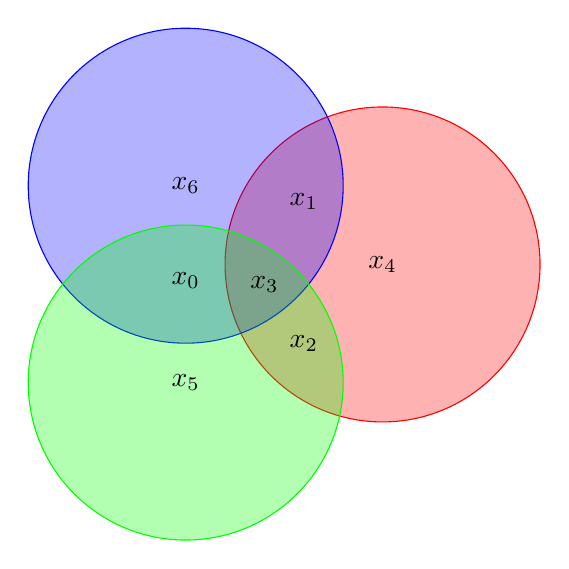
\begin{tikzpicture}
        % Círculo para x4 (x1, x2, x3) - vermelho com transparência
        \fill[red, opacity=0.3] (2,0) circle (2);
        \draw[red] (2,0) circle (2); %node at (2,2.5) {$x_4$};
        \node at (2,0) {$x_4$};

        % Círculo para x5 (x0, x2, x3) - azul com transparência
        \fill[blue, opacity=0.3] (-0.5,1) circle (2);
        \draw[blue] (-0.5,1) circle (2); %node at (-0.5,3.5) {$x_5$};
        \node at (-0.5,1) {$x_6$};

        % Círculo para x6 (x0, x1, x3) - verde com transparência
        \fill[green, opacity=0.3] (-0.5,-1.5) circle (2);
        \draw[green] (-0.5,-1.5) circle (2); %node at (-0.5,-4) {$x_6$};
        \node at (-0.5,-1.5) {$x_5$};

        % Rótulos para as interseções
        \node at (0.50,-0.25) {$x_3$}; % Interseção dos três círculos (x3)
        \node at (-0.5,-0.2) {$x_0$}; % Interseção x5 e x6 (x0, x3)
        \node at (1,-1) {$x_2$}; % Interseção x4 e x6 (x1, x3)
        \node at (1,0.8) {$x_1$}; % Interseção x4 e x5 (x2, x3)
    \end{tikzpicture}
    \caption{Diagrama de Venn para o código de Hamming (7,4,3). 
    Cada círculo representa uma verificação de paridade: 
    $x_4$ cobre $x_1, x_2, x_3$, $x_5$ cobre $x_0, x_2, x_3$, e 
    $x_6$ cobre $x_0, x_1, x_3$. 
    As interseções mostram os bits compartilhados entre as verificações.}
    \label{fig:hamming_venn}
\end{figure}

As $2^4 = 16$ palavras-código são os vetores no espaço nulo de $\mathbf{H}$,
$C = \{x : \mathbf{H} x = 0 \}$, sendo eles elencados a seguir:
        \begin{equation}
        \begin{matrix}
        0000000 & 0100101 & 1000011 & 1100110 \\
        0001111 & 0101010 & 1001100 & 1101001 \\
        0010110 & 0110011 & 1010101 & 1110000 \\
        0011001 & 0111100 & 1011010 & 1111111
        \end{matrix} 
        \end{equation}

Note que o código é fechado em relação à soma e à subtração.
Se $v_1, v_2 \in C$ então $\mathbf{H} (v_1 + v_2) = \mathbf{H} v_1 + \mathbf{H} v_2 = 0$, desta forma, $v_1 + v_2 \in C$. 
Da mesma forma também temos $v_1 - v_2 \in C$, uma vez que soma e subtração
módulo 2 são equivalentes.

A distância mínima do código é $d_{\text{min}} = 3$, igual ao peso mínimo, que é o menor
número de 1s em uma palavra-código não nula. Para verificar, note que não
existem palavras-código com peso 1 ou 2.
Primeiramente, para peso 1, veja que uma palavra com um único 1 na posição $i$ não
satisfaz $\mathbf{H} \mathbf{x} = \mathbf{0}$, pois não existe coluna nula em $\mathbf{H}$. 
Para obter $\mathbf{H} \mathbf{x} = \mathbf{0}$, sendo $\mathbf{x}$ não nulo apenas na posição $i$,
deveríamos ter a $i$-ésima coluna de $\mathbf{H}$ nula, o que não ocorre.
Vejamos agora o próximo caso, peso 2. Note que a soma de duas colunas de $\mathbf{H}$ (módulo 2) nunca é zero,
pois todas as colunas são distintas e não nulas.
Por fim, podemos verificar que existem palavras com peso 3, como $(0,0,1,0,0,1,1)$, que satisfazem $\mathbf{H} \mathbf{x} = \mathbf{0}$.
Como a distância de Hamming entre duas palavras $\mathbf{v}_1, \mathbf{v}_2 \in C$ 
é o peso de $\mathbf{v}_1 + \mathbf{v}_2$ (outra palavra-código), 
a distância mínima é igual ao peso mínimo, $d_{\text{min}} = 3$.

Pelo \hyperref[thm:deteccaoerros]{teorema de detecção de erros}\index{teorema!de detecção de erros}, o código detecta até $d - 1 = 2$ erros. 
Pelo \hyperref[thm:correcaoerros]{teorema de correção de erros}\index{teorema!de correção de erros}, ele corrige até $\lfloor (d - 1)/2 \rfloor = \lfloor 2/2 \rfloor = 1$ erro por palavra-código. 
Isso torna o código de Hamming (7,4,3) ideal para canais onde erros únicos são mais prováveis, 
como em um canal binário simétrico (BSC) com baixa probabilidade de erro.



\subsection{Decodificação por Síndrome}
Para corrigir erros, usamos a \emph{decodificação por síndrome}\index{código!decodificação por síndrome}\index{código!síndrome}. 
Seja $\mathbf{x}$ a palavra-código transmitida e $\mathbf{y} = \mathbf{x} + \mathbf{z}$ 
a palavra recebida, onde $\mathbf{z}$ é o vetor de erro (com 1s nas posições erradas). 
A síndrome é calculada como:
\begin{equation}
\mathbf{s} = \mathbf{H} \mathbf{y} = \mathbf{H} (\mathbf{x} + \mathbf{z}) = \mathbf{H} \mathbf{x} + \mathbf{H} \mathbf{z} = \mathbf{H} \mathbf{z},
\end{equation}
pois $\mathbf{H} \mathbf{x} = \mathbf{0}$ para $\mathbf{x} \in C$. 
A síndrome $\mathbf{s}$ depende apenas do erro $\mathbf{z}$. 
Se $\mathbf{s} = \mathbf{0}$, assumimos que não houve erro (ou houve um erro indetectável, com probabilidade baixa).
Se $\mathbf{s} \neq \mathbf{0}$ e assumindo um erro de 1 bit na posição $i$, 
teremos $\mathbf{s} = \mathbf{h}_i$, a $i$-ésima coluna de $\mathbf{H}$.
Como as colunas de $\mathbf{H}$ são todas distintas e não nulas, podemos identificar $i$,
a posição do bit errôneo e corrigi-lo.

\begin{example}
Suponha que a palavra recebida seja $\mathbf{y}^T = (0,1,1,1,0,0,1)$, 
que não é uma palavra-código válida. Calculamos a síndrome:
\begin{equation}
\mathbf{H} \mathbf{y} = \begin{pmatrix}
0 & 1 & 1 & 1 & 1 & 0 & 0 \\
1 & 0 & 1 & 1 & 0 & 1 & 0 \\
1 & 1 & 0 & 1 & 0 & 0 & 1
\end{pmatrix} 
\begin{pmatrix} 0 \\ 1 \\ 1 \\ 1 \\ 0 \\ 0 \\ 1 \end{pmatrix} = \begin{pmatrix} 1 + 1 + 1 \\ 1 + 1 \\ 1 + 1 + 1 \end{pmatrix} \mod 2 = \begin{pmatrix} 1 \\ 0 \\ 1 \end{pmatrix}.
\end{equation}
A síndrome $\mathbf{s} = (1,0,1)^T$ corresponde à coluna 2 de $\mathbf{H}$ (indexada de 0 a 6, coluna $\mathbf{h}_1$). 
Isso indica um erro na posição 2 (bit $y_1$). Corrigimos definindo $\mathbf{z} = (0,1,0,0,0,0,0)$, e calculamos:
\begin{equation}
\mathbf{x} = \mathbf{y} + \mathbf{z} = (0,1,1,1,0,0,1) + (0,1,0,0,0,0,0) = (0,0,1,1,0,0,1).
\end{equation}
Verificamos que $\mathbf{x} = (0,0,1,1,0,0,1)$ é uma palavra-código válida, pois:
\begin{equation}
\mathbf{H} \mathbf{x} = \begin{pmatrix} 0 + 1 + 1 \\ 0 + 1 + 1 \\ 0 + 1 + 1 \end{pmatrix} \mod 2 = \begin{pmatrix} 0 \\ 0 \\ 0 \end{pmatrix}.
\end{equation}
Os bits de dados são $(x_0, x_1, x_2, x_3) = (0,0,1,1)$.
\end{example}

O procedimento de decodificação por síndrome é esquematizado da seguinte forma:
\begin{enumerate}[itemsep=0pt, topsep=0pt, parsep=0pt, partopsep=0pt]
    \item Calcule a síndrome $\mathbf{s} = \mathbf{H} \mathbf{y}$.
    \item Se $\mathbf{s} = \mathbf{0}$, assuma $\mathbf{z} = \mathbf{0}$ e vá ao passo \ref{itm:xyplusz}.
    \item Caso contrário, identifique a coluna $\mathbf{h}_i$ de $\mathbf{H}$ igual a $\mathbf{s}$, e defina $\mathbf{z}$ com 1 na posição $i$ e 0s nas demais.
    \item\label{itm:xyplusz} Calcule $\mathbf{x} = \mathbf{y} + \mathbf{z}$.
    \item Retorne os bits de dados $(x_0, x_1, x_2, x_3)$.
\end{enumerate}
Esse procedimento corrige exatamente um erro por palavra-código, mas falha se
houver dois ou mais erros, pois a síndrome pode apontar para uma correção
incorreta.

\subsection{Propriedades e Aplicações}

O código de Hamming (7,4,3) tem $2^4 = 16$ palavras-código, correspondendo 
às combinações lineares das colunas de $\mathbf{G}$. A matriz $\mathbf{H}$ 
tem posto 3, e seu espaço nulo tem dimensão $7 - 3 = 4$, confirmando as 
$2^4$ palavras. Isso segue do Teorema do Posto-nulidade\index{teorema!posto-nulidade}, que afirma que, 
para uma matriz $m \times n$, o posto somado à dimensão do espaço nulo 
(nulidade) é igual ao número de colunas: $\text{posto} + \text{nulidade} = n $\footnote{
O posto de uma matriz é a dimensão do espaço vetorial gerado por suas colunas (ou linhas), 
representando o número de linhas ou colunas linearmente independentes. 
A nulidade é a dimensão do espaço nulo, o conjunto de vetores $\mathbf{x}$ 
tais que $\mathbf{A} \mathbf{x} = \mathbf{0}$, ou seja, o número de soluções
independentes para o sistema homogêneo.}. 
Assim, com $n = 7$ e posto 3, a nulidade é 4. 
A probabilidade de erro indetectável em um canal binário simétrico (BSC) 
com probabilidade de erro $p$ é limitada por:
\begin{equation}
P_u(E) \leq 2^{-(n-k)} [1 - (1-p)^n] = 2^{-3} [1 - (1-p)^7],
\end{equation}
o que indica que a adição de 3 bits de paridade reduz significativamente os erros indetectáveis \parencite{costello2004}.



Para entender por que o código de Hamming (7,4,3) é eficiente, precisamos
introduzir o conceito de esfera de Hamming e o limite de Hamming, que
determina o número máximo de palavras-código para um dado nível de correção de
erros.

\begin{definition}[Esfera de Hamming]
Uma \emph{esfera de Hamming}\index{código!esfera de Hamming} de raio $t$ centrada em uma sequência $\mathbf{x}$ de $n$ 
símbolos em um alfabeto $q$-ário é o conjunto de todas as sequências $\mathbf{y}$ 
tais que a distância de Hamming $d_H(\mathbf{x}, \mathbf{y}) \leq t$. 
Formalmente:
\begin{equation}
B(\mathbf{x}, t) = \{ \mathbf{y} \in \{0, 1, \dots, q-1\}^n : d_H(\mathbf{x}, \mathbf{y}) \leq t \}.
\end{equation}
O volume ou número de sequências em uma esfera de raio $t$ é dado por:
\begin{equation}
|B(\mathbf{x}, t)| = \sum_{i=0}^{t} \binom{n}{i} (q-1)^i,
\end{equation}
onde $\binom{n}{i}$ é o número de maneiras de escolher $i$ posições para alterar, 
e $(q-1)^i$ é o número de escolhas para cada uma das $i$ posições 
(podemos escolher $q-1$ símbolos diferentes do original em cada posição).
\end{definition}

Para um código binário ($q = 2$), temos $(q-1)^i = 1$, e para $t = 1$, o tamanho da esfera é:
\begin{equation}
\sum_{i=0}^{1} \binom{n}{i} = \binom{n}{0} + \binom{n}{1} = 1 + n.
\end{equation}
Por exemplo, com $n = 7$, uma esfera de raio 1 contém $1 + 7 = 8$ sequências: 
a palavra-código e as 7 sequências que diferem dela em exatamente 1 bit.

\begin{theorem}[Limite de Hamming]\index{código!limite de Hamming}
Um código $q$-ário de comprimento $n$ que corrige até $t$ erros pode ter no máximo
$\sfrac{q^n}{|B(\mathbf{x}, t)|}$ palavras-código, ou seja:
\begin{equation}
|B(\mathbf{x}, t)| \cdot \vert \mathcal{C} \vert \leq q^n,
\end{equation}
onde $\vert \mathcal{C} \vert$ é o número de palavras-código, e 
$|B(\mathbf{x}, t)| = \sum_{i=0}^{t} \binom{n}{i} (q-1)^i$ é o tamanho de uma esfera de Hamming 
de raio $t$. Um código que atinge a igualdade é chamado de código perfeito\footnote[][-2cm]{
Um código perfeito é um código que atinge o limite de Hamming com igualdade, ou seja, 
as esferas de Hamming de raio $t$ centradas nas palavras-código são disjuntas e cobrem 
exatamente todas as $q^n$ sequências possíveis. Isso maximiza o número de palavras-código 
para um dado nível de correção de erros, sem deixar lacunas ou sobreposições no espaço de sequências.}.
\end{theorem}

\begin{proof}
Para corrigir até $t$ erros, cada sequência recebida deve ser decodificada para
uma única palavra-código. Isso implica que as esferas de Hamming de raio $t$
centradas nas palavras-código devem ser disjuntas: se $\mathbf{c}_1$ e
$\mathbf{c}_2$ são palavras-código distintas, então 
$B(\mathbf{c}_1, t) \cap B(\mathbf{c}_2, t) = \emptyset$. 
Caso contrário, uma sequência $\mathbf{y} \in B(\mathbf{c}_1, t) \cap B(\mathbf{c}_2, t)$
estaria a distância $\leq t$ de duas palavras-código, impossibilitando a correção única.

Cada esfera $B(\mathbf{c}_i, t)$  contém $\sum_{i=0}^{t} \binom{n}{i} (q-1)^i$ sequências.
Se o código tem $\vert \mathcal{C} \vert$ palavras-código, 
o número total de sequências cobertas pelas esferas é:
\begin{equation}
\vert \mathcal{C} \vert \cdot |B(\mathbf{c}_i, t)| = \vert \mathcal{C} \vert \cdot \sum_{i=0}^{t} \binom{n}{i} (q-1)^i.
\end{equation}
O número total de sequências possíveis de $n$ símbolos é $q^n$. 
Como as esferas são disjuntas e cada sequência pertence a no máximo uma esfera, temos:
\begin{equation} 
\vert \mathcal{C} \vert \cdot \sum_{i=0}^{t} \binom{n}{i} (q-1)^i \leq q^n.
\end{equation}
Se a igualdade for atingida, as esferas cobrem exatamente todas as $q^n$ sequências, e o código é perfeito.
\end{proof}

Apliquemos o teorema ao código de Hamming (7,4,3). 
Ele é um código binário $q = 2$ com $n = 7$, $k = 4$, e $d = 3$, 
que corrige $t = \lfloor (d-1)/2 \rfloor = 1$ erro. 
O número de palavras-código é $\vert \mathcal{C} \vert = 2^k = 2^4 = 16$, 
e o tamanho de uma esfera de raio $t = 1$ é:
\begin{equation}
\sum_{i=0}^{1} \binom{7}{i} (2-1)^i = \binom{7}{0} + \binom{7}{1} = 1 + 7 = 8.
\end{equation}
Substituímos no limite de Hamming:
\begin{equation}
|B(\mathbf{x}, 1)| \cdot \vert \mathcal{C} \vert = 8 \cdot 16 = 128 \leq 2^7 = 128.
\end{equation}
A igualdade indica que o código de Hamming (7,4,3) é perfeito: 
as esferas de Hamming de raio 1 centradas nas 16 palavras-código cobrem exatamente 
todas as $2^7 = 128$ sequências possíveis de 7 bits, otimizando a correção de erros
sem deixar lacunas ou sobreposições.


Códigos da família de Hamming, como o (7,4,3) e o (31,26,3), são amplamente
utilizados em sistemas onde a confiabilidade é crítica, incluindo memórias de
computadores (e.g., ECC RAM) e comunicações digitais. O código (7,4,3),
proposto por Richard Hamming, corrige 1 erro e detecta 2 erros com uma
sobrecarga de aproximadamente 43\% de bits de paridade, sendo um marco teórico
e histórico, especialmente nos primeiros sistemas computacionais, como o IBM 701. Já o código
(31,26,3), com sobrecarga de cerca de 16\%, é mais comum em memórias RAM
modernas, protegendo blocos de 32 bits com eficiência, ideal para cenários onde
erros de bit único predominam, como em chips DRAM. Sua estrutura linear e
decodificação eficiente, baseada na abordagem por síndrome, estabeleceram os
códigos Hamming como uma base para o desenvolvimento de códigos mais avançados,
como os códigos BCH e Reed-Muller, que oferecem maior capacidade de correção,
porém com maior complexidade e overhead.






\section{Construção dos Códigos de Hamming}

Os códigos de Hamming\index{código!de Hamming} formam uma família de códigos lineares que podem ser
gerados de maneira sistemática com base na representação binária das posições
dos bits. Essa construção permite determinar os bits de paridade e os bits de
dados de forma algorítmica, garantindo uma distância mínima $d_{\text{min}} = 3$, que
corrige 1 erro e detecta 2 erros. Abaixo, descrevemos o processo de construção.

A ideia central é associar cada posição de bit a uma representação binária e
usar os bits de paridade para verificar subconjuntos específicos de posições,
determinados pelos bits 1 na representação binária. As posições são numeradas
de 1 a $n$, e os bits de paridade são colocados em posições que são
potências de 2 (1, 2, 4, 8, etc.), enquanto os bits de dados ocupam as demais
posições.

\begin{table*}[h]
    \centering
    {%
    \footnotesize%
    \setlength{\tabcolsep}{4pt}
    \begin{tabular}{|*{22}{c|}}
        \multicolumn{2}{ c }{ \ }  & \rot{1} & \rot{10} & \rot{11} & \rot{100} & \rot{101} & \rot{110} & \rot{111} & \rot{1000} & \rot{1001} & \rot{1010} & \rot{1011} & \rot{1100} & \rot{1101} & \rot{1110} & \rot{1111} & \rot{10000} & \rot{10001} & \rot{10010} & \rot{10011} & \rot{10100} \\
        \hline
        \multicolumn{2}{ |c| }{posição do bit} & 1 & 2 & 3 & 4 & 5 & 6 & 7 & 8 & 9 & 10 & 11 & 12 & 13 & 14 & 15 & 16 & 17 & 18 & 19 & 20 \\ \hline 
        \multicolumn{2}{ |c| }{bits de dado codificados} & \cellcolor{blue!25} \( p_1 \) & \cellcolor{red!25} \( p_2 \) & \( p_3 \) & \cellcolor{green!25} \( p_4 \) & \( p_5 \) & \( p_6 \) & \( p_7 \) & \cellcolor{yellow!25} \( p_8 \) & \( p_9 \) & \( p_{10} \) & \( p_{11} \) & \( p_{12} \) & \( p_{13} \) & \( p_{14} \) & \( p_{15} \) & \cellcolor{orange!25} \( p_{16} \) & \( p_{17} \) & \( p_{18} \) & \( p_{19} \) & \( p_{20} \) \\ \hline 
        \multirow{5}{*}{\rotatebox[origin=c]{90}{ \parbox[c]{5em}{Cobertura dos bits de paridade}}} 
            & \cellcolor{blue!25} \( p_1 \) & X &   & X &   & X &   & X &   & X &   & X &   & X &   & X &   & X &   & X & \\ \cline{2-22}
            & \cellcolor{red!25} \( p_2 \) &   & X & X &   &   & X & X &   &   & X & X &   &   & X & X &   &   & X & X & \\ \cline{2-22} 
            & \cellcolor{green!25} \( p_4 \) &   &   &   & X & X & X & X &   &   &   &   & X & X & X & X &   &   &   &   & X \\ \cline{2-22}
            & \cellcolor{yellow!25} \( p_8 \) &   &   &   &   &   &   &   & X & X & X & X & X & X & X & X &   &   &   &   & \\ \cline{2-22}
            & \cellcolor{orange!25} \( p_{16} \) &   &   &   &   &   &   &   &   &   &   &   &   &   &   &   & X & X & X & X & X \\
        \hline
    \end{tabular}
    }
    \caption{Tabela de construção de um código de Hamming com até 20 bits. As posições marcadas com \( p_i \) são bits de paridade, e as demais são bits de dados. A cobertura de cada bit de paridade é determinada pela presença de 1 na posição correspondente na representação binária.}
    \label{tab:hamming_construction}
\end{table*}

O algoritmo de construção segue estas regras:
\begin{itemize}[itemsep=0pt, topsep=0pt, parsep=0pt, partopsep=0pt]
    \item As posições dos bits de paridade são $2^0 = 1$), $2^1 = 2$, $2^2 = 4$, $2^3 = 8$, etc.,
      e são denotadas por $p_1, p_2, p_4, p_8, \ldots$.
    \item Cada bit de paridade $p_i$ (onde $i = 2^j$ para algum $j$) cobre as posições
      cuja representação binária tem um 1 na posição $j+1$ (contando de 1 a partir do 
      bit menos significativo). Por exemplo:
    \begin{itemize}[itemsep=0pt, topsep=0pt, parsep=0pt, partopsep=0pt]
        \item $p_1$ (posição 1): cobre posições com 1 no primeiro bit, como 1 (\textbf{1}), 3 (1\textbf{1}), 5 (10\textbf{1}), 7 (11\textbf{1}), etc.
        \item $p_2$ (posição 2): cobre posições com 1 no segundo bit, como 2 (\textbf{1}0), 3 (\textbf{1}1), 6 (1\textbf{1}0), 7 (1\textbf{1}1), etc.
        \item $p_4$ (posição 4): cobre posições com 1 no terceiro bit, como 4 (\textbf{1}00), 5 (\textbf{1}01), 6 (\textbf{1}10), 7 (\textbf{1}11), etc.
        \item E assim por diante...
    \end{itemize}
    \item Os bits de paridade são calculados para garantir que a soma (módulo 2) 
      dos bits que eles cobrem seja zero, satisfazendo as equações de verificação.
    \item As posições restantes são ocupadas pelos bits de dados.
\end{itemize}

Se utilizarmos $m$ bits de paridade, as posições totais cobertas vão de 1 a $2^m - 1$, 
pois essas são todas as combinações possíveis com $m$ bits. 
Subtraindo os $m$ bits de paridade, o número de bits de dados é $2^m - 1 - m$. 
A distância mínima do código resultante é $d = 3$, 
permitindo correção de 1 erro e detecção de 2 erros. 
Variando $m$, obtemos a família de códigos de Hamming, como mostrado na tabela a seguir:

\begin{table*}[h]
    \small
    \begin{tabular}{lllll}
      \toprule
      \multicolumn{1}{>{\raggedright\arraybackslash}p{1.5cm}}{bits de paridade} & 
      \multicolumn{1}{>{\raggedright\arraybackslash}p{1.5cm}}{total de bits} & 
      \multicolumn{1}{>{\raggedright\arraybackslash}p{1.5cm}}{bits de dados} & nome & taxa \\ 
      \midrule
        2 & 3  & 1  & Hamming(3,1)  & $1/3 \approx 0.333$  \\ 
        3 & 7  & 4  & Hamming(7,4)  & $4/7 \approx 0.571$  \\ 
        4 & 15 & 11 & Hamming(15,11) & $11/15 \approx 0.733$ \\ 
        5 & 31 & 26 & Hamming(31,26) & $26/31 \approx 0.839$ \\ 
      \bottomrule
    \end{tabular}
    \caption{Variações da família de códigos de Hamming para diferentes valores 
    de $m$, com $n = 2^m - 1$ e $k = 2^m - 1 - m$. A taxa $R = k/n$ indica a eficiência do código.}
    \label{tab:hamming_variations}
\end{table*}

Por exemplo, para $m = 3$, temos $n = 2^3 - 1 = 7$ bits totais, 
com 3 bits de paridade (posições 1, 2, 4) e 4 bits de dados (posições 3, 5, 6, 7), 
resultando no código Hamming(7,4). Para $m = 5$, $n = 2^5 - 1 = 31$, 
com 5 bits de paridade e 26 bits de dados, formando o Hamming(31,26).

Essa construção sistemática permite gerar códigos de Hamming para diferentes
tamanhos de dados, equilibrando redundância e capacidade de correção, e serve
como base para entender códigos lineares mais complexos.

